\documentclass[fleqn]{article}
\usepackage{amsmath, amssymb, amsthm}
\usepackage{fullpage}
\usepackage{listings}
\usepackage{stix}
\usepackage[utf8]{inputenc}
\usepackage{tikz}
\usetikzlibrary{arrows.meta, positioning}
\lstset{ basicstyle=\ttfamily, }

\newcommand{\SMN}{$s$\nobreakdash-$m$\nobreakdash-$n$}

\begin{document}

\begin{center}
{\Large \textbf{Homework 4 - Categorical}}\\[0.5em]
{\large 6\nobreakdash-1.8(1)(a)--(i) Reduction Pyramids}
\end{center}

\bigskip

\noindent\textbf{The reduction pyramid.}\quad Each undecidability proof in 1.8(1) can have the same shape. Let $A$ be a problem already known to be undecidable, let $B$ be the problem of interest, and let $\mathbf{2} = \{0, 1\}$. A many-one reduction is a total computable function $k$ such that, for every $x$,
\[
x \in A \iff k(x) \in B.
\]
We arrange these data as a pyramid:

\bigskip

\begin{center}
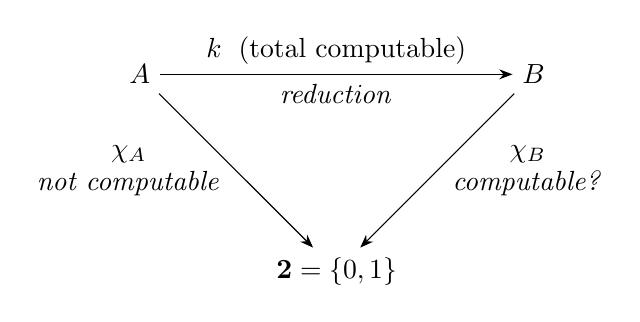
\begin{tikzpicture}[>=Stealth, node distance=2.5cm]
  \node (A) at (0, 2.5)  {$A$};
  \node (B) at (5, 2.5)  {$B$};
  \node (Two) at (2.5, 0) {$\mathbf{2} = \{0, 1\}$};
  \draw[->] (A) -- node[above] {$k$ \;(total computable)} node[below] {\textit{reduction}} (B);
  \draw[->] (A) -- node[left, xshift=-2pt]  {\shortstack{$\chi_A$ \\ \textit{not computable}}} (Two);
  \draw[->] (B) -- node[right, xshift=2pt] {\shortstack{$\chi_B$ \\ \textit{computable?}}} (Two);
\end{tikzpicture}
\end{center}

\bigskip

\noindent The reduction $k$ makes the triangle commute:
\[
\chi_A \;=\; \chi_B \circ k.
\]
The left edge $\chi_A \colon A \to \mathbf{2}$ is the characteristic function of the known undecidable problem. Typically by theorem 6\nobreakdash-1.1, $\chi_A$ is \textit{not} computable. $k$ is built (usually via the $s$\nobreakdash-$m$\nobreakdash-$n$ theorem) so that it is an `isomorphism of decision problems' under the equivalence
\[
x \in A \iff k(x) \in B.
\]
The right edge $\chi_B$ is the candidate decision procedure for the harder problem. If it existed as a computable function, then by composition $\chi_B \circ k$ would be a computable characteristic function for $A$, contradicting the left edge. Hence $\chi_B$ cannot be computable: $B$ is undecidable.

This pyramid is exactly the schema applied throughout; the only data that change between exercises are $A$ and $k$, the starting point and the reduction.

\bigskip

\noindent\textbf{Drawn out (a)}\quad We instantiate the pyramid for part (a): $x \in E_x$

\smallskip

$A = \,$`$x \in W_x$'

$B = \,$`$x \in E_x$'

\medskip

\textit{Construct $k$.}\quad Define
\[
f(x, y) \simeq
\begin{cases}
y & \text{if } x \in W_x, \\
\text{undefined} & \text{otherwise.}
\end{cases}
\]
$f$ is computable. The \SMN theorem yields a total computable $k$ with $\phi_{k(x)}(y) \simeq f(x, y)$. Inspection gives
\[
x \in W_x \implies E_{k(x)} = \mathbb{N}, \qquad x \notin W_x \implies E_{k(x)} = \varnothing,
\]
so in particular $x \in W_x \iff k(x) \in E_{k(x)}$.

\medskip

\textit{Pyramid.}

\begin{center}
\begin{tikzpicture}[>=Stealth]
  \node (A) at (0, 2.5)  {`$x \in W_x$'};
  \node (B) at (6, 2.5)  {`$x \in E_x$'};
  \node (Two) at (3, 0) {$\{0, 1\}$};
  \draw[->] (A) -- node[above] {$k$} (B);
  \draw[->] (A) -- node[left, xshift=-2pt]  {$\chi_A$} (Two);
  \draw[->] (B) -- node[right, xshift=2pt] {$\chi_B$} (Two);
\end{tikzpicture}
\end{center}

The triangle commutes by $(*)$: $\chi_A(x) = \chi_B(k(x))$. The left edge is non-computable (theorem 6\nobreakdash-1.1). If the right edge were computable, the composite along the hypotenuse and right edge would compute the left edge, a contradiction. Hence `$x \in E_x$' is undecidable. \qed

\bigskip

\noindent\textbf{Filling (b)--(i).}\quad In each row below, the pyramid has the same shape; only $A$ and $k$ change. For the Rice cases the role of $k$ is played by the reduction supplied in the proof of Rice's theorem (theorem 6\nobreakdash-1.7) for the appropriate class $\mathscr{B}$.

\medskip

\noindent\textbf{(b)}\quad $B = \,$`$W_x = W_y$', $A = \,$`$\phi_x$ is total', $k(x) = (x, c)$ where $c$ is a fixed index of $\mathbf{0}$.

Since $W_c = \mathbb{N}$, we have $\phi_x$ total $\iff W_x = \mathbb{N} \iff W_x = W_c$, i.e.\ $x \in A \iff k(x) \in B$.

\medskip

\noindent\textbf{(c)}\quad $B = \,$`$\phi_x(x) = 0$', $A = \,$`$x \in W_x$', $k$ the \SMN reduction with $\phi_{k(x)}(y) \simeq f(x, y)$.

Define
\[
f(x, y) \simeq \begin{cases} 0 & x \in W_x, \\ \text{undef.} & \text{otherwise.} \end{cases}
\]
Then $\phi_{k(x)}(k(x)) = 0 \iff x \in W_x$, i.e.\ $x \in A \iff k(x) \in B$.

\medskip

\noindent\textbf{(d)}\quad $B = \,$`$\phi_x(y) = 0$', $A = \,$`$x \in W_x$', $k'(x) = (k(x), c)$ for any fixed $c$, with $k$ as in (c).

By construction of $k$, $\phi_{k(x)}(c) = 0 \iff x \in W_x$, so $x \in A \iff k'(x) \in B$.

\medskip

\noindent\textbf{(e)}\quad $B = \,$`$x \in E_y$', $A = \,$`$c \in E_y$' for fixed $c$, $k(y) = (c, y)$.

The equivalence $y \in A \iff k(y) \in B$ is immediate from the definitions.

\medskip

\noindent\textbf{(f)}\quad $B = \,$`$\phi_x$ is total and constant', $A = \,$`$x \in W_x$', $k$ the reduction produced by the proof of Rice's theorem for $\mathscr{B}_f = \{$total constant functions$\}$ with $g = \mathbf{0} \in \mathscr{B}_f$.

$\mathscr{B}_f$ contains $\mathbf{0}$ and omits the identity, so $\varnothing \neq \mathscr{B}_f \neq \mathscr{C}_1$ and the Rice reduction applies.

\medskip

\noindent\textbf{(g)}\quad $B = \,$`$W_x = \varnothing$', $A = \,$`$x \in W_x$', $k$ the reduction from Rice's theorem for $\mathscr{B}_g = \{ f_\varnothing \}$.

Via $W_x = \mathrm{Dom}(\phi_x)$, membership in $\mathscr{B}_g$ corresponds to the predicate `$W_x = \varnothing$'; the singleton is nonempty and a proper subclass of $\mathscr{C}_1$, satisfying the Rice hypotheses.

\medskip

\noindent\textbf{(h)}\quad $B = \,$`$E_x$ is infinite', $A = \,$`$x \in W_x$', $k$ the reduction from Rice's theorem for $\mathscr{B}_h = \{ f \in \mathscr{C}_1 : \mathrm{Ran}(f) \text{ infinite} \}$.

$\mathscr{B}_h$ contains the identity and omits $\mathbf{0}$, so $\varnothing \neq \mathscr{B}_h \neq \mathscr{C}_1$ and the Rice reduction applies.

\medskip

\noindent\textbf{(i)}\quad $B = \,$`$\phi_x = g$' for $g$ a fixed computable function, $A = \,$`$x \in W_x$', $k$ the reduction from Rice's theorem for $\mathscr{B}_i = \{g\}$.

$\mathscr{C}_1$ contains computable functions distinct from $g$, so $\varnothing \neq \mathscr{B}_i \neq \mathscr{C}_1$ and the Rice reduction applies.

\end{document}
